\chapter{State of Art}
This chapter presents an overview of the concepts and technologies that were studied and used on the development of this work. 
In section \textit{2.1 - Software Quality}, will be presented general aspects of software quality such as \textit{quality measurement},  \textit{software metrics}, \textit{program analysis} and some tools that are used in this area.  

Section \textit{2.2 - Java and OSGi} will introduce OSGi a framework for build service oriented Java modular applications as well the motivation 
behind this solution and why standard quality metrics aren't sufficient for this kind of application. 


\section{Software Quality}

There has been many definitions of software quality(TODO REF - Metrics and Models in Software Quality Engineering) and there is even an ISO norm for it, the ISO/IEC 25010(TODO REF). All this definitions agree that the main motivation to perform continuous software quality management is to avoid \textbf{software failures} and increase \textbf{maintainability} in the sense that the more quality a program has the easier will be to maintain and the less bugs or abnormal behavior it will have and the more it will conform with its functional and non functional requirements that can be simply defined as \textit{what} the software does and \textit{how} the software will do respectively. 

Another important aspect of software quality is that it can be divided in two groups, the \textbf{external} and \textbf{internal} quality. When we talk about \textit{external quality} we are aiming to the user view which is the one that sees the software working and use it, this kind of quality is usually enforced through software testing. External quality can also be mapped to functional requirements so the greater external quality is the more usable and less defects it will have for example. The opposite is internal or structural quality that aims to how the software is architect-ed internally which is the perspective of the programmer and non functional requirements so the higher internal quality the better the code is structured, efficient, robust and maintainable it should be. Image 2.1 illustrates internal and external quality and its target audience.


\begin{figure}[h]
\caption{Internal and external quality audience}
\centering
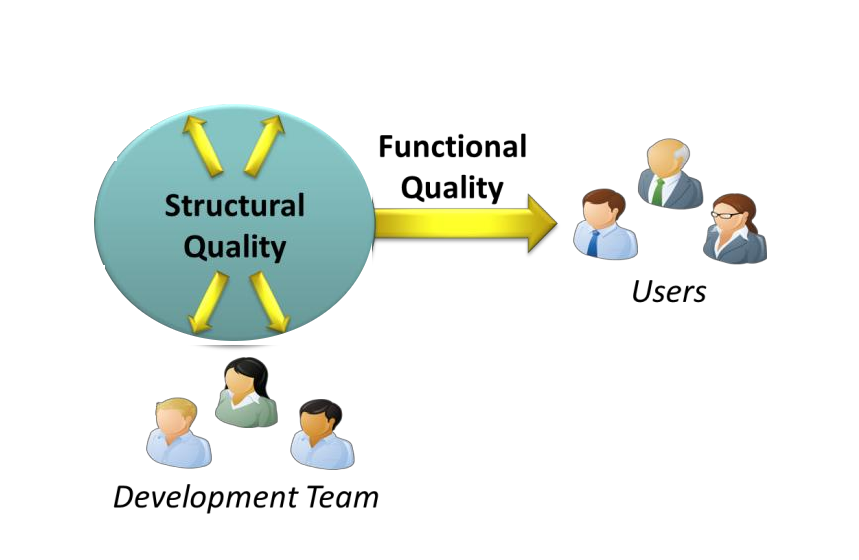
\includegraphics[scale=0.5]{external-internal-quality}
\end{figure}

% functional quality(performed via automated testing)
% structural quality(\textbf{this is where our work shines})

\subsection{Quality Measurement}
Quality measurement focuses on quantifying software desirable characteristics and each characteristic can have a set of measurable attributes, for example \textit{high cohesion} is a desirable characteristic and \textit{LOC - lines of code} is a measurable attribute related to cohesion. Quality measurement is close related to internal quality and in most cases is performed via static code analysis where program code is inspected to search for quality attributes to be measured but in some cases a dynamic analysis, where the program analysis is done during software execution, can be performed to measure characteristics that can be perceived only when software is running, for example performance or usability.     

In the extent of this work the characteristics of software to be considered and measured later are listed and described in table 2.1:  

\begin{table}[h]
\caption{Quality characteristics to be considered}
\begin{center}
    \begin{tabular}{  p{3cm} | p{8cm} | p{5cm} }
    \hline
    Characteristic & Description & OSGi example \\  \hline
    Reliability & the degree to which a system or component performs its required functions under stated conditions for a specified period of time. & Stale service references.\\ \hline
    Performance Efficiency & Performance relative to the amount of resources used under stated conditions for a specified
period of time. & Bundle startup time, also bundle dependency can decrease performance. \\ \hline
    Security & the degree of protection of information and data so that unauthorized persons or systems cannot read, access or modify them. & Bundle declares permission \\ \hline
    Maintainability & The degree to which the product can be modified. & Modules should be loosely coupled, bundles should publish only interfaces etc. \\ 
    \hline
     
    \end{tabular}
    Source: \cite{cisq 2012}
\end{center}
\end{table}
\FloatBarrier

\subsection{Software Metric}
A software metric is the measurement of a software attribute which in turn is a quantitative calculation of a characteristic.
\subsubsection{Common Software Metrics}
The table 2.2 below shows some well known software metrics and its description:

\begin{table}[h]
\caption{Common Software metrics}
\begin{center}
    \begin{tabular}{  p{3cm} | p{8cm} }
    \hline
    Metric & Description \\  \hline
    Cyclomatic complexity & It is a quantitative measure of the complexity of programming instructions.\\ \hline
    Cohesion & measure the dependency between units of code like for example classes in object oriented programing or modules in modular programming like OSGi. \\ \hline
    Coupling & measures how well two software components are data related or how dependent they are. \\ \hline
    Lines of code (LOC) & used to measure the size of a computer program by counting the number of lines in the text of the program's source code. \\ \hline
    Code coverage &  measures the code lines that are executed for a given set of software tests \\ \hline
    Function point analysis (FPA) & used to measure the size (functions) of software. \\
    \hline

    \end{tabular}
    \\*Source: \cite{sqa 2012}
\end{center}
\end{table}

\FloatBarrier

\subsection{Program Analysis}
Program analysis is the process of automatically analyzing the behavior of computer programs. Two main approaches in program analysis are \textbf{static program analysis} and \textbf{dynamic program analysis}. Main applications of program analysis are program correctness, program optimization and \textit{quality measurement}.

\subsubsection{Static Program Analysis}
 Is the analysis of computer software that is performed without actually executing programs \citep{Wichmann 1995}.  

\subsubsection{Dynamic Program Analysis}

\subsection{Quality Analysis Tools}
This section will list most used code quality analysis tools.

\section{Java and OSGi}
I the context of Java modular applications...
